

\begin{figure}[h!]
    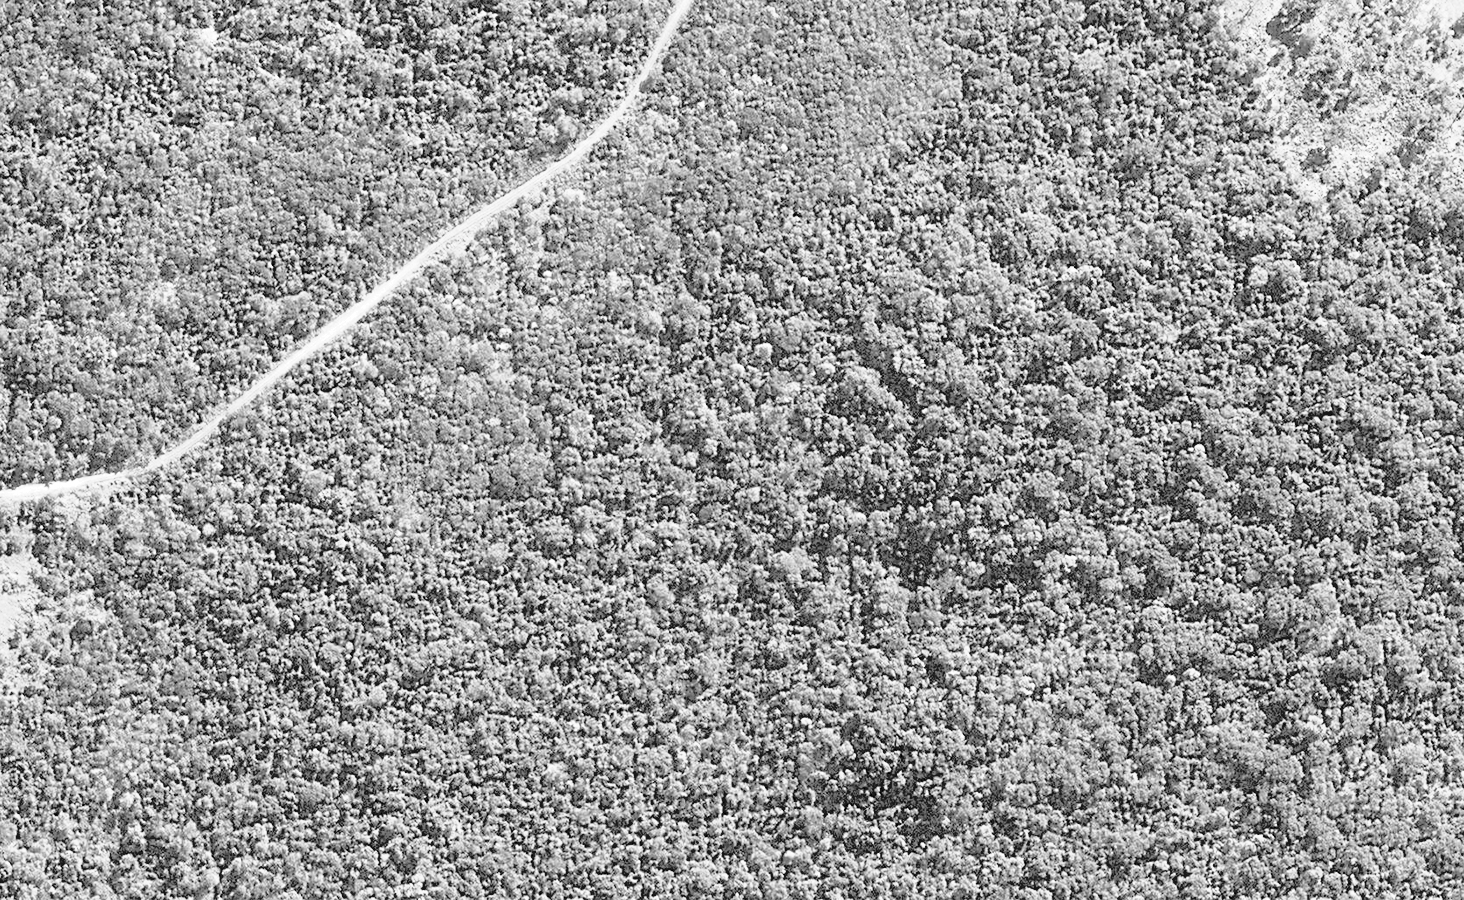
\includegraphics[width=\textwidth]{Imagenes/Homomorfico/ST2.png}
     \hfill
     \caption{Imagen aérea (satelital) de reserva privada Sombra de Toro (identificada como ST2 en la tabla), en escala de grises. Resolución de imagen de 1464 x 900 píxeles, resolución espacial de 0,5 m por pixel.}
    \label{sombratorogris}
\end{figure}

\begin{figure}[h!]
    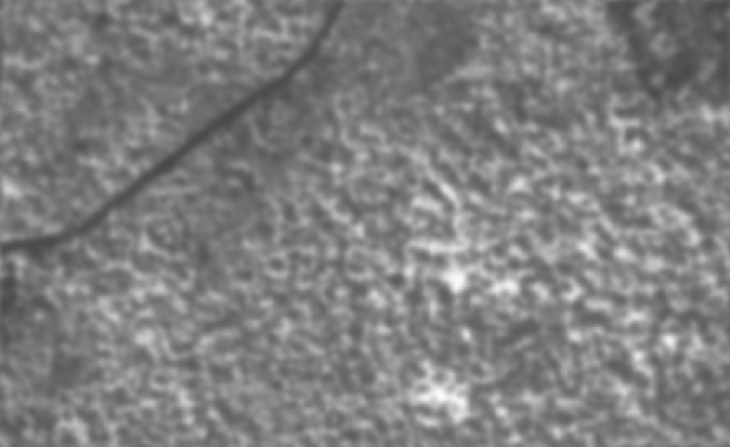
\includegraphics[width=\textwidth]{Imagenes/Homomorfico/ST2_filtro.png}
     \hfill
     \caption{Imagen filtrada aplicando el filtro homomórfico a la imagen de la figura \ref{sombratorogris}.}
    \label{ST filtro}
\end{figure}

\begin{figure}[h!]
    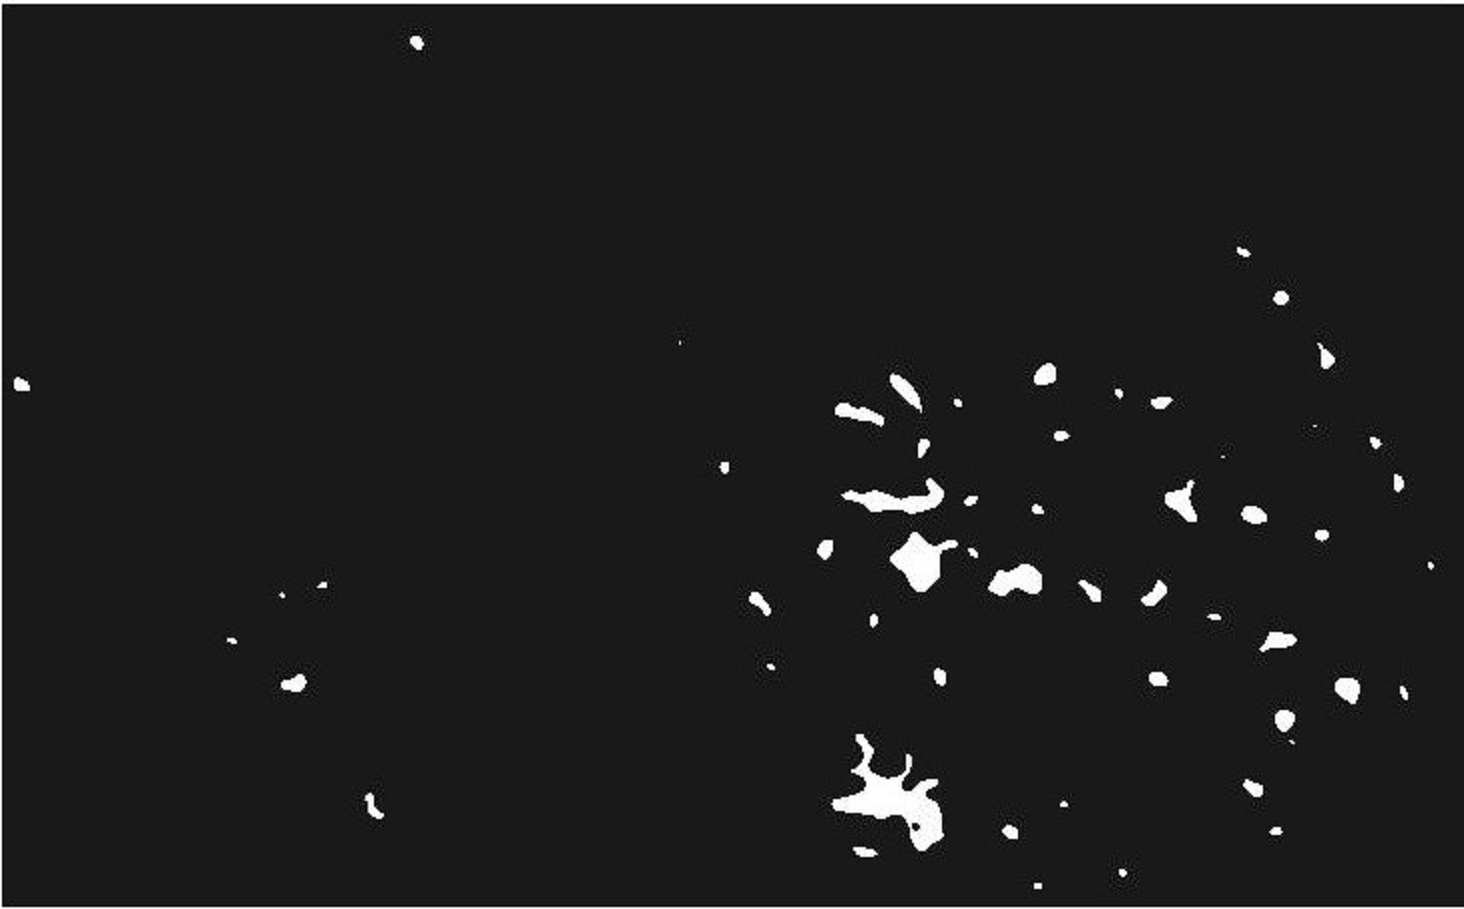
\includegraphics[width=\textwidth]{Imagenes/Homomorfico/ST2_bin.png}
     \hfill
     \caption{Máscara binaria obtenida a partir de la imagen de la figura \ref{sombratorogris} con umbral de 0,45.}
    \label{mascaraST}
\end{figure}

\begin{figure}[h!]
    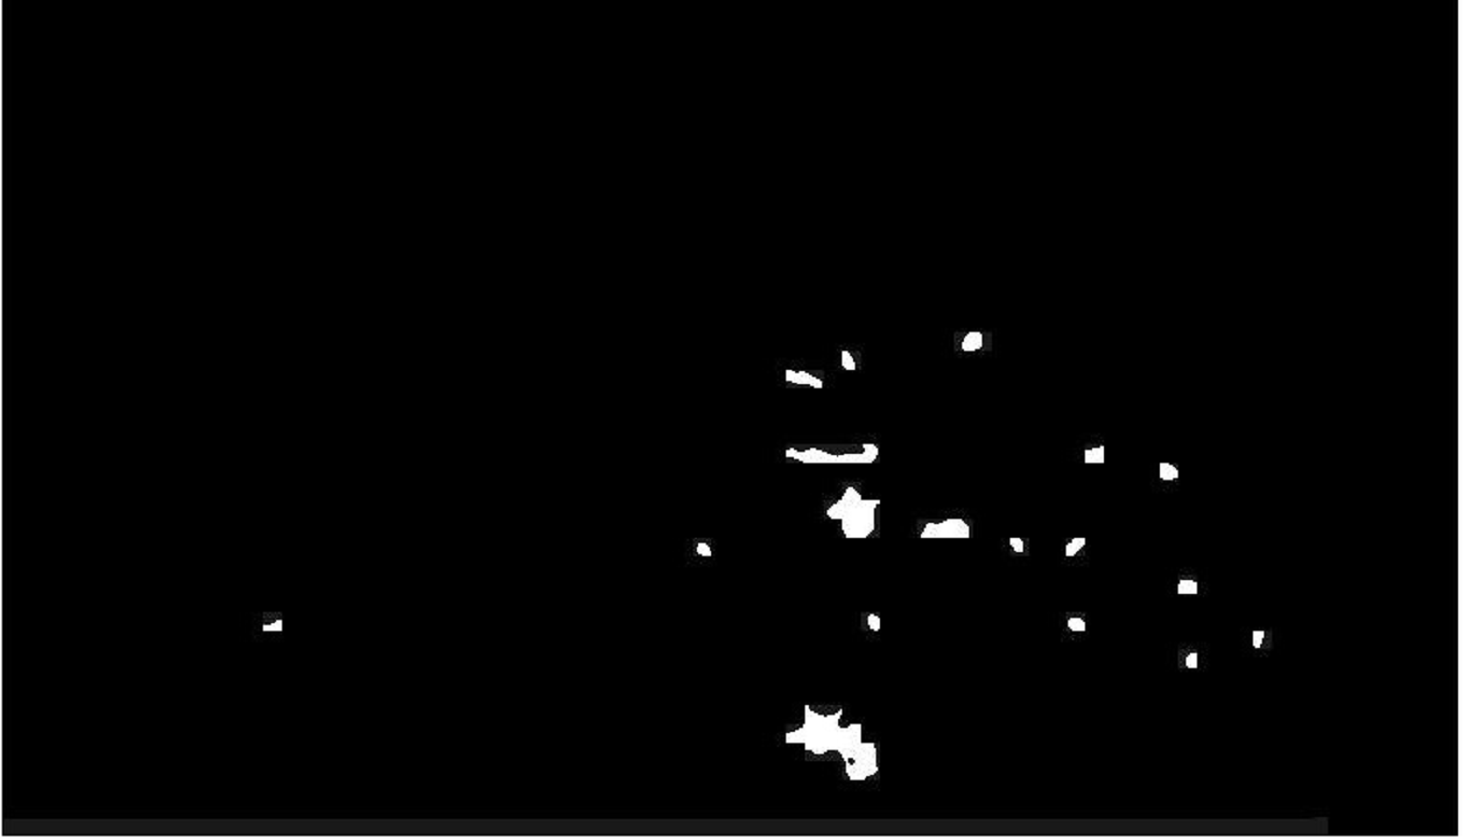
\includegraphics[width=\textwidth]{Imagenes/Homomorfico/ST2_masked.png}
     \hfill
     \caption{Sombras seleccionadas por el algoritmo a partir de la imagen de la figura \ref{mascaraST}.}
    \label{seleccionadaST}
\end{figure}

\begin{figure}[h!]
    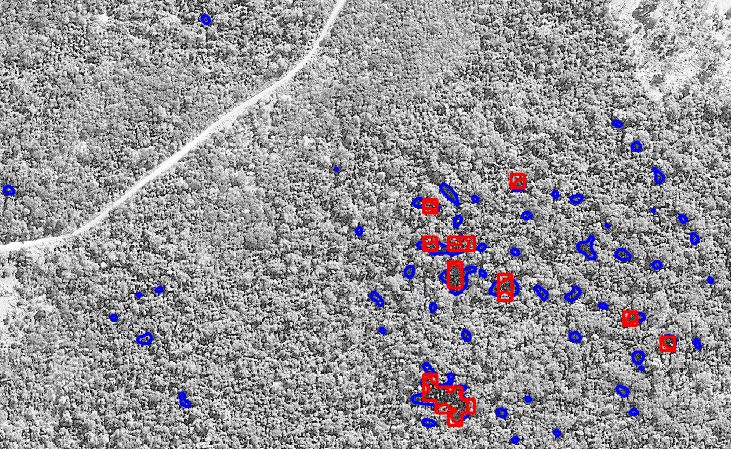
\includegraphics[width=\textwidth]{Imagenes/Homomorfico/ST2_25.png}
     \hfill
     \caption{Superposición de máscara binaria (contorno azul) y máscaras seleccionadas por ventana deslizante (contorno rojo) a la imagen original.}
    \label{ST25}
\end{figure}
%%%%%%%%%%%%%%%%%%%%%%%%%%%%%%%%%%%%%%%%%%%%%%%%%%%%%%%%%%%%%%%%%%%%%%%%%%%%%%%%
\begin{figure}[h!]
    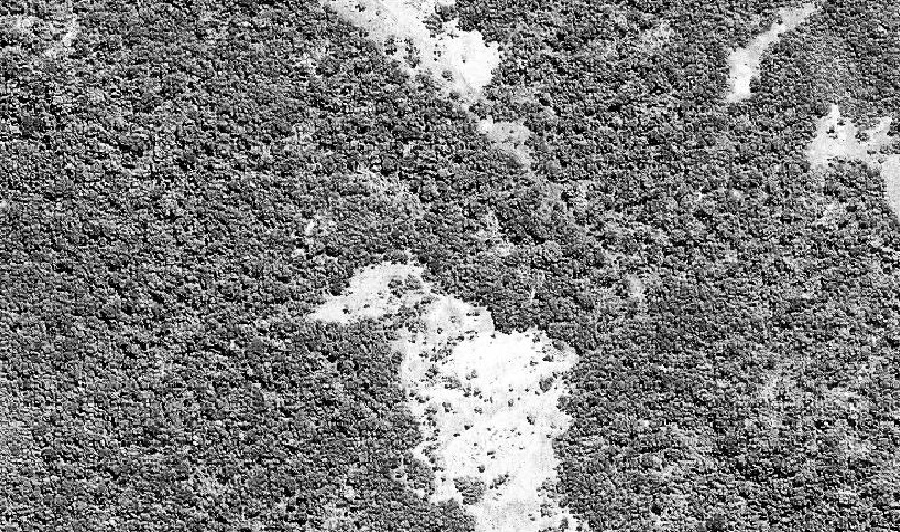
\includegraphics[width=\textwidth]{Imagenes/Homomorfico/PS1_original.jpg}
     \hfill
     \caption{Imagen aérea (satelital) de reserva Parque de la Sierra (identificada como PS1 en la tabla), en escala de grises. Resolución de imagen de 1464 x 900 píxeles, resolución espacial de 0,5 m por pixel.}
    \label{PS1}
\end{figure}

\begin{figure}[h!]
    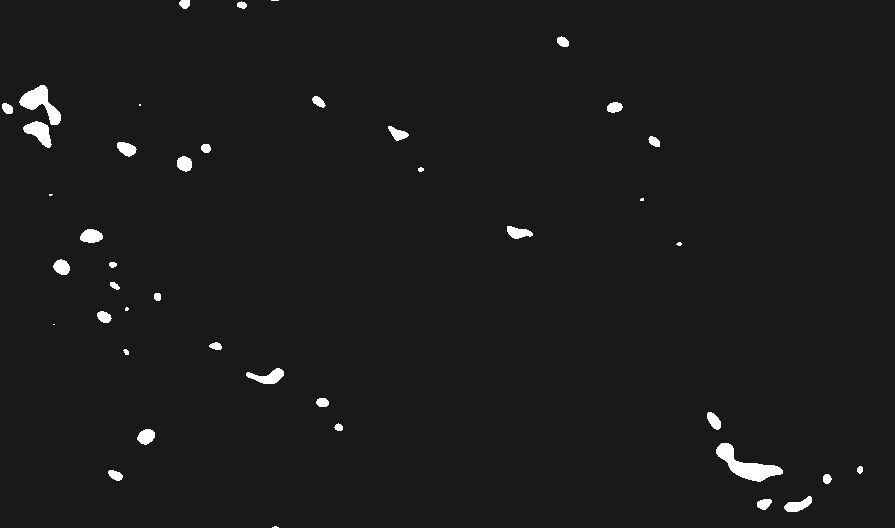
\includegraphics[width=\textwidth]{Imagenes/Homomorfico/PS1_bin.png}
     \hfill
     \caption{Máscara binaria obtenida a partir de la imagen de la figura \ref{PS1} con umbral de 0,45.}
    \label{mascaraPS1}
\end{figure}

\begin{figure}[h!]
    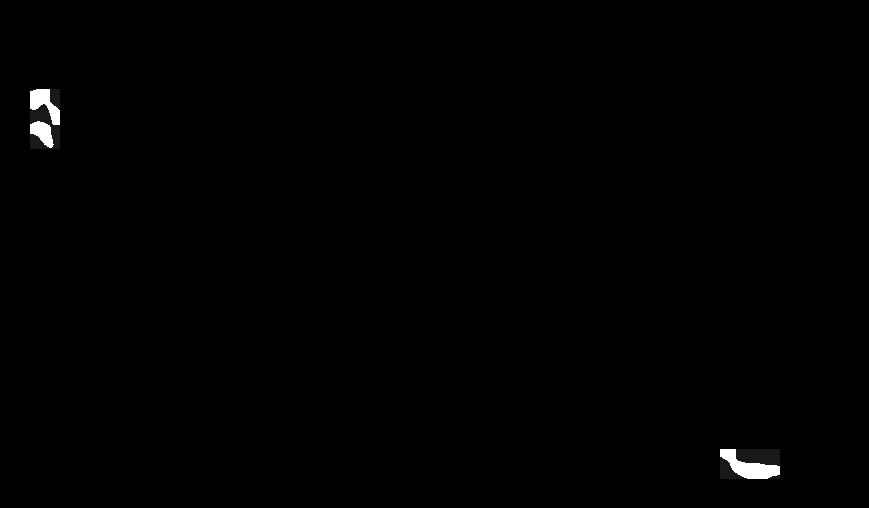
\includegraphics[width=\textwidth]{Imagenes/Homomorfico/PS1_masked.png}
     \hfill
     \caption{Sombras seleccionadas por el algoritmo a partir de la imagen de la figura \ref{mascaraPS1}.}
    \label{seleccionadaPS1}
\end{figure}